% SPDX-License-Identifier: Apache-2.0 OR MIND-UCAL-1.0
% © James Ross Ω FLYING•ROBOTS <https://github.com/flyingrobots>
\documentclass[tikz,border=10pt]{standalone}
\usepackage{tikz}
\usetikzlibrary{positioning,arrows.meta,calc,fit,shadows}

\begin{document}
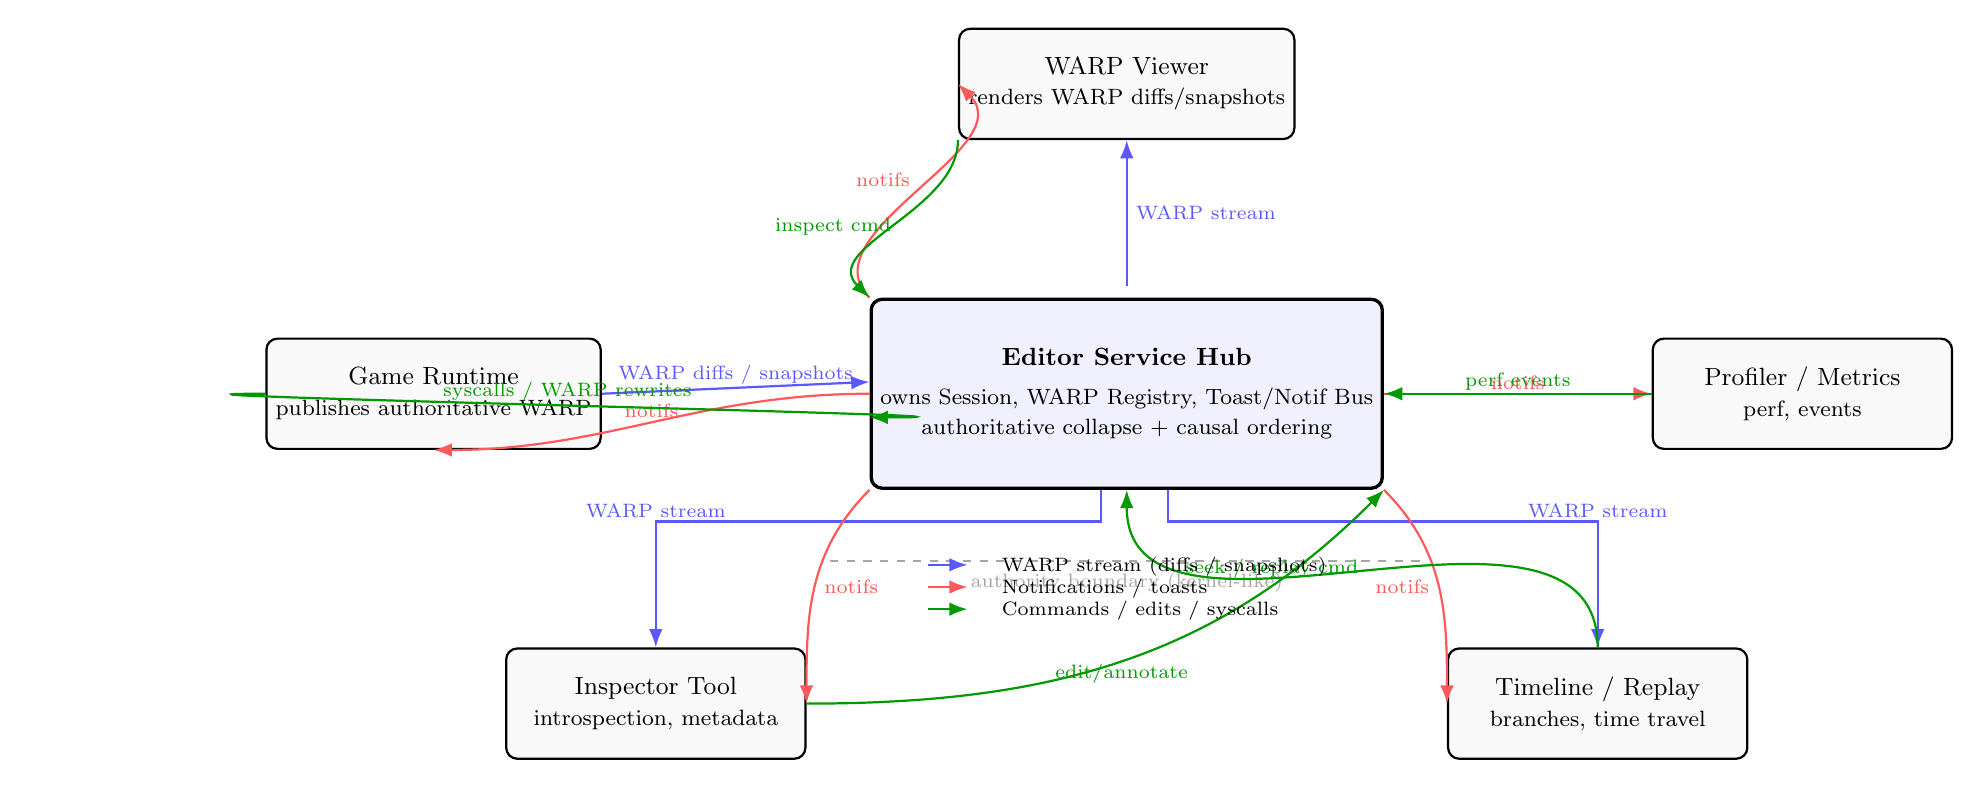
\begin{tikzpicture}[
  >=Latex,
  font=\small,
  node distance=1.8cm,
  svc/.style={draw, rounded corners, thick, align=center, minimum width=3.8cm, minimum height=1.4cm, fill=gray!5},
  hub/.style={draw, rounded corners, very thick, align=center, minimum width=5.2cm, minimum height=2.4cm, fill=blue!6},
  warpstream/.style={->, thick, blue!65},
  notif/.style={->, thick, red!65},
  cmd/.style={->, thick, green!60!black},
  boundary/.style={dashed, thick, gray!70},
  lbl/.style={font=\scriptsize, inner sep=1pt},
]

% Editor Service Hub
\node[hub] (hub) {
  \textbf{Editor Service Hub}\\[3pt]
  \footnotesize owns Session, WARP Registry, Toast/Notif Bus\\
  \footnotesize authoritative collapse + causal ordering
};

% Tools around the hub
\node[svc, above=2.0cm of hub] (viewer) {WARP Viewer\\\footnotesize renders WARP diffs/snapshots};
\node[svc, below left=2.0cm and 0.8cm of hub] (inspector) {Inspector Tool\\\footnotesize introspection, metadata};
\node[svc, below right=2.0cm and 0.8cm of hub] (timeline) {Timeline / Replay\\\footnotesize branches, time travel};
\node[svc, left=3.4cm of hub] (game) {Game Runtime\\\footnotesize publishes authoritative WARP};
\node[svc, right=3.4cm of hub] (profiler) {Profiler / Metrics\\\footnotesize perf, events};

% Service authority boundary (logical)
\draw[boundary] ($(hub.south west)+(-0.5,-0.9)$) -- ($(hub.south east)+(0.5,-0.9)$)
  node[midway, below=3pt, lbl, fill=white] {authority boundary (kernel-like)};

% WARP Streams (blue)
\draw[warpstream] (game.east) -- node[lbl, above] {WARP diffs / snapshots} ($(hub.west)+(0,0.15)$);
\draw[warpstream] ($(hub.north)+(0,0.15)$) -- node[lbl, right=2pt] {WARP stream} (viewer.south);
\draw[warpstream] ($(hub.south west)!0.45!(hub.south east)$) -- ++(0,-0.4) -| node[lbl, above] {WARP stream} (inspector.north);
\draw[warpstream] ($(hub.south west)!0.58!(hub.south east)$) -- ++(0,-0.4) -| node[lbl, above] {WARP stream} (timeline.north);

% Notifications (red)
\draw[notif] (hub.north west) to[out=135,in=-45] node[lbl, above left] {notifs} (viewer.west);
\draw[notif] (hub.west) to[out=180,in=0] node[lbl, above] {notifs} (game.south);
\draw[notif] (hub.south west) to[out=225,in=90] node[lbl, right=2pt] {notifs} (inspector.east);
\draw[notif] (hub.south east) to[out=315,in=90] node[lbl, left=2pt] {notifs} (timeline.west);
\draw[notif] (hub.east) -- node[lbl, above] {notifs} (profiler.west);

% Commands back to hub (green)
\draw[cmd] (viewer.south west) to[out=-90,in=135] node[lbl, left] {inspect cmd} (hub.north west);
\draw[cmd] (inspector.east) to[out=0,in=225] node[lbl, below] {edit/annotate} (hub.south east);
\draw[cmd] (timeline.north) to[out=90,in=-90] node[lbl, left] {seek / replay cmd} (hub.south);
\draw[cmd] (profiler.west) to[out=180,in=0] node[lbl, above] {perf events} (hub.east);
\draw[cmd] (game.west) to[out=180,in=0] node[lbl, above] {syscalls / WARP rewrites} ($(hub.west)+(0,-0.3)$);

% Optional: label the outer pattern
\node[below=0.8cm of hub, lbl] {
  \begin{tabular}{@{}ll@{}}
    \tikz{\draw[warpstream] (0,0)--(0.5,0);} & WARP stream (diffs / snapshots)\\
    \tikz{\draw[notif] (0,0)--(0.5,0);} & Notifications / toasts\\
    \tikz{\draw[cmd] (0,0)--(0.5,0);} & Commands / edits / syscalls
  \end{tabular}
};

\end{tikzpicture}
\end{document}
